\chapter{Algunos elementos}

En este capítulo se describen algunas particularidades de la plantilla, y se proporcionan algunos ejemplos con elementos de uso frecuente. No se comentan aspectos comunes relacionados con el uso de \LaTeX, ya que existe gran cantidad de información al respecto.

\section{Configuración}
La configuración es muy sencilla. Al margen de la adaptación particular que pueda hacerse, la elaboración de un documento solamente requiere información relativa al autor, título y tutores. Ésta ha de configurarse en el archivo \verb+include\opciones.tex+.  \\

Además, en el archivo \verb+include\colores.tex+ puede configurarse el color \verb+tema+, utilizado en títulos, elementos flotantes y, opcionalmente, tablas y negritas. Por defecto, se recomienda ponerlo a \verb+{0,0,0}+  (negro). Pueden escribirse \bft{negritas con el color configurado} con el comando \verb+\bft{texto}+. \\

Por último, en el archivo principal se pueden configurar las fuentes utilizadas en la portada, preámbulo y documento.

\section{Colores}


En el archivo \verb+include\colores.tex+ se predefinen algunos colores. También varios comandos para utilizar negritas con ellos. En concreto, se proporcionan cinco: Con el comando \verb+\bfa{texto}+ se pueden poner las cosas en negrita \bfa{azul}. Con el comando \verb+\bfr{texto}+ se pueden poner las cosas en negrita \bfr{rojo}.Con el comando \verb+\bfn{texto}+ se pueden poner las cosas en negrita \bfn{naranja}. Con el comando \verb+\bfv{texto}+ se pueden poner las cosas en negrita \bfv{verde}. Con el comando \verb+\bfm{texto}+ se pueden poner las cosas en negrita \bfm{mostaza}.\\

\begin{itemize}
\item [\hmarkr] No es conveniente abusar los colores, salvo en alguna ocasión adicional. Por ejemplo, si el color del tema es {\bf negro} o \bfa{azul} se puede utilizar el \bfr{rojo} para alguna advertencia.
\end{itemize}

\section{Listas y enumeraciones}

El entorno \textit{itemize} usa, por defecto, el color del tema. Los símbolos utilizados para marcar los items están pre-definidos en el archivo de configuración, y pueden cambiarse. También es posible seleccionar, mediante \verb+\item[símbolo]+ el símbolo específico para cada línea. Esta lista muestra los símbolos por defecto:

\begin{itemize}
\item Primer ítem
\begin{itemize}
\item Primer ítem en el segundo nivel
\item Otro ítem en el segundo nivel
\begin{itemize}
\item Ítem en el tercer nivel
\end{itemize}
\end{itemize}
\item Segundo ítem
\item Tercer ítem \\
\end{itemize}

En esta se usan algunos caracteres especiales predefinidos para marcar los ítems. Existen comandos para mostrar algunos de estos caracteres con los colores azul, rojo y el color del tema.

\begin{itemize}
\item[\vmarka] \verb+\vmarka+ : ``v'' representa el símbolo, y ``a'' el color
\item[\xmarkr] \verb+\xmarkr+
\item[\lmarkt] \verb+\lmarkt+ : el color ``t'' corresponde al tema.
\item[\hmarkt] \verb+\hmarkt+ 
\item[\fmarkt] \verb+\fmarkt+ \\
\end{itemize}

Las enumeraciones también están preconfiguradas en el archivo de configuración:

\begin{enumerate}
\item Esto es una enumeración
\item Con algunos elementos adicionales
\item Que se pueden quitar
\end{enumerate}

Pueden ser modificadas, como en el siguiente ejemplo.

\begin{enumerate}[labelindent=\parindent ,leftmargin=*,label=\mbox{\bft{[Re \arabic*]}}]
\setcounter{enumi}{7}
\item Esto es una enumeración
\item Sin elementos
\item Adicionales
\end{enumerate}


\section{Elementos flotantes}

En el archivo de \verb+include\configuracion+ existen varios parámetros que se fijan en la configuración para figuras y tablas, pero se pueden alterar de manera ocasional (y excepcional) al maquetar el documento. La mayoría son relativos al título, y se pueden cambiar a través de las funcionalidades que proporciona el paquete \verb+caption+. Cuando se cambian para un elemento particular \bft{es buena práctica restaurar el valor original}, para que el documento tenga un aspecto uniforme.

\begin{verbatim}
% Títulos
\DeclareCaptionFont{tema}{\color{tema}} % Color
\captionsetup{labelfont={tema, bf}}     % Estilo
\captionsetup{font=normalsize}          % Tamaño
\captionsetup{width=.9\linewidth}       % Anchura del título
 % Distancia de la figura al texto.
\setlength{\intextsep}{1cm} 
\setlength{\textfloatsep}{1cm}         
\end{verbatim}

\subsection{Tablas}
Las tablas se hacen de modo normal, aunque se ha añadido la capacidad utilizar celdas que ocupen múltiples filas, colores en los encabezados, y anchuras fijas. Se recomienda mirar el código fuente de la tabla \ref{tab:mod1}.\\

Con respecto al color de los encabezados, es conveniente utilizar el mismo en todo el documento. Una opción con respecto al fondo del encabezado es utilizar el mismo que el del texto pero con transparencia. \\



% --------------------------------------------------
% Esto es para poner colores en las asignaturas
% en el ejemplo concreto
\newcommand{\bi}{\bfn{ES}/\bfr{EN}}
\newcommand{\esp}{\bfn{ES}}
\newcommand{\eng}{\bfr{EN}}
% --------------------------------------------------

\begin{table}[h]\footnotesize
\renewcommand{\arraystretch}{1.3} % Altura
\begin{center}
\begin{tabular}{|L{2.5cm}| L{3cm}| C{6cm} c | c |} % Tres primeras con anchura predefinida
\hline 
\rowcolor{tema!10} % Color con transparencia correspondiente
\bft{Módulo I} & \bft{Materia} & \multicolumn{2}{|c|}{\bft{Asignatura}}& \bft{ECTS} \\ \hline 

\multirow{9}{2.5cm}{Formación Básica (60 ECTS)} & % Aquí se indica que esta ocupa nueve filas.
\multirow{4}{3cm}{Fundamentos Matemáticos de la Informática} & 
Álgebra y Matemática Discreta & \esp  & 6 \\ \cline{3-5} 
& & Cálculo y Métodos Numéricos & \bi  & 6 \\ \cline{3-5} 
& & Estadística & \bi  & 6 \\ \cline{3-5}
& & Lógica& \esp  & 6 \\ \cline{2-5}
& Fundamentos Físicos de la Informática & Fundamentos Físicos de la Informática & \bi  & 6 \\ \cline{2-5}
& \multirow{2}{3cm}{Ingeniería de Computadores} & 
Estructura de Computadores & \esp  & 6 \\ \cline{3-5} 
& & Tecnología de Computadores & \esp  & 6 \\ \cline{2-5} 
& \multirow{2}{3cm}{Programación} & 
Fundamentos de Programación I & \esp  & 6 \\ \cline{3-5} 
& & Fundamentos de Programación II & \bi  & 6 \\ \cline{2-5}
%& \makecell[cl]{Gestión de las \\ Organizaciones} & Fundamentos de Gestión Empresarial & \esp  & 6 \\ \hline 
& Gestión de las \mbox{Organizaciones} & Fundamentos de Gestión Empresarial & \esp  & 6 \\ \hline 
\end{tabular}
\end{center}
\caption[Asignaturas del Módulo I]{Asignaturas del Módulo I.}
\label{tab:mod1}
\renewcommand{\arraystretch}{1} 
\end{table}

\subsection{Figuras}

Con respecto a las figuras, a veces es utilizar un texto descriptivo demasiado ancho puede ser antiestético. Por ejemplo en la \ref{fig:esiiabI} el rótulo ocupa toda la línea\footnote{Por defecto, ocupa el 90\%, que es el valor por defecto en la configuración, pero se ha cambiado para que se vea mejor el efecto.}. En la figura \ref{fig:esiiabII} se corrige este efecto con:

\begin{verbatim}
\begin{figure}[b] 
\captionsetup{width=0.8\linewidth}
...
\end{verbatim}

Después, se restaura el valor original de la configuración:
\begin{verbatim}
...
\captionsetup{width=0.9\linewidth}
\end{figure}
\end{verbatim}


\begin{figure}[p] 
\captionsetup{width=1\linewidth}
\begin{center}
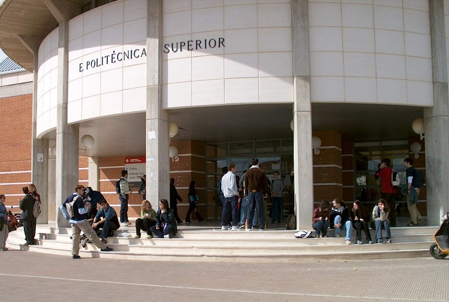
\includegraphics[width=10cm]{figs/esiiab.png}
\end{center}
\caption[Escuela Superior de Ingeniería Informática I]{Escuela Superior de Ingeniería Informática. Esto es un texto descriptivo algo más largo que puede producir un efecto feo.}
\label{fig:esiiabI}
\end{figure}



\begin{figure}[p] 
\captionsetup{width=0.8\linewidth}
\begin{center}
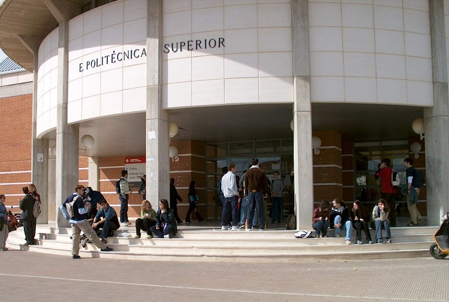
\includegraphics[width=10cm]{figs/esiiab.png}
\end{center}
\caption[Escuela Superior de Ingeniería Informática II]{Escuela Superior de Ingeniería Informática. Esto es un texto descriptivo algo más largo que puede producir un efecto feo.}
\label{fig:esiiabII}
\captionsetup{width=0.9\linewidth}
\end{figure}

Se incluye el paquete \verb+subfigure+ para la inclusión de figuras con varias imágenes o gráficas, como la que muestra la figura \ref{fig:subfiguras}.
\begin{figure}[htb]
\begin{center}
\begin{subfigure}[b]{0.4\linewidth}
\begin{center}
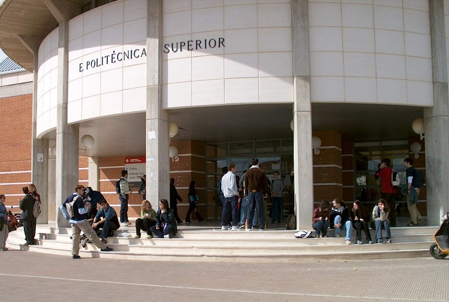
\includegraphics[width=0.9\linewidth]{figs/esiiab.png}
\caption{Fotografía de la izquierda}\label{fig:esiiabIII}
\end{center}
\end{subfigure} 
\begin{subfigure}[b]{0.4\linewidth}
\begin{center}
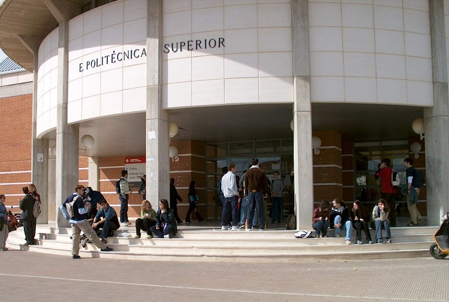
\includegraphics[width=0.9\linewidth]{figs/esiiab.png}
\caption{Fotografía de la drecha}\label{fig:esiiabIV}
\end{center}
\end{subfigure} 
\end{center}
\caption[Ejemplo de subfiguras]{Ejemplo de inclusión de subfiguras}
\label{fig:subfiguras}
\end{figure}



\section{Algoritmos y código}

Con respecto a los algoritmos (pseudocódigo) y código pueden implementarse, respectivamente, mediante el uso de los paquetes \verb+algorithmic+ y \verb+listings+. Pueden configurarse ambos entornos el archivo \verb+include\configuracion+. Por otra parte, se han definido dos entornos flotantes, denominados \verb+algorithm+ y \verb+code+ para encapsular y mostrar ambos tipos de elemento de manera uniforme.\\


El algoritmo \ref{alg:search} muestra un ejemplo de pseudocódigo. Se han añadido dos comandos, \verb+\va{variable}+ para distinguir las \va{variables}, y \verb+\fu{funcion}+ para distinguir las \fu{Funciones}. \\



\begin{algorithm}[b]
\begin{algorithmic}[1]
 	\Function{Tree-Search}{ }
 	\State \va{open} $\leftarrow$ \Call{CreateNode}{\fu{Initial-State}} \Comment{Creates the root}
	\While {\va{open} $\neq \emptyset$}
		\State \va{node} $\leftarrow$ \Call{Extract}{\va{open}}
		\If {\Call{TestGoal}{\va{node.STATE}}}
			\State \Return \Call{RecoverPath}{\va{node}} \Comment{Solution found}
		\EndIf		
				
		\State \va{successors} $\leftarrow$ \Call{Expand}{\va{node}}
		\ForAll {\va{successor} \bft{en} \va{successors}} \Comment{Processes each successor }
			\State  \Call{Insert}{\va{successor, open}}
		\EndFor	
	\EndWhile
	\State \Return failure \Comment{No solution have been found}
 	\EndFunction
\end{algorithmic}
\caption{Tree-Search exploration}
\label{alg:search}
\end{algorithm}

Por último, el listado \ref{alg:code} muestra el código del algoritmo \ref{alg:search} en \textit{Python}. El paquete \verb+listings+  contiene multitud de opciones para el manejo de distintos lenguajes y para personalización.

\begin{code}
\begin{lstlisting}

def search(initial):
	open = [initial]
	while open:
		node = open.pop()
		if testGoal(node):
			return recoverPath(node)
		successors = expand(node)
		for succesor in successors:
			open.append(succesor)
	return failure
		
\end{lstlisting}
\caption{Ejemplo de código en Python}
\label{alg:code}
\end{code}


\section{Bibliografía}

Esto es una cita \cite{RUSSELL} y esto otra \cite{AlphaZero}. La bibliografía se gestiona con bibtex y un estilo predefinido. No se han hecho modificaciones de momento.

\section{Notación matemática}

Utiliza las fuentes por defecto del tema, aunque también se pueden cambiar.


\[
J(\theta)=\frac{1}{2m}\left[ \sum_{i=1}^m\left(h_\theta(x^{(i)})-y^{(i)}\right)^2 + \lambda \sum_{j=1}^n \theta_j^2 \right], \mbox{ } \lambda >0
\]

